\begin{frame}
\begin{columns}[t]
\begin{column}{0.5\textwidth}
\begin{block}{\textbf{3-simplex}}
H-representation
\begin{equation*}
\begin{aligned}\label{eq:simplex3H}
1 &\geq x_1 + x_2 + x_3\\
x_1 &\geq 0\\
x_2 &\geq 0\\
x_3 &\geq 0
\end{aligned}
\end{equation*}
V-representation
$$
\begin{bmatrix}
  1 & 0 & 0 & 0\\
  1 & 1 & 0 & 0\\
  1 & 0 & 1 & 0\\
  1 & 0 & 0 & 1\\
\end{bmatrix}
$$
\end{block}
\end{column}
\begin{column}{0.5\textwidth}
\begin{center}
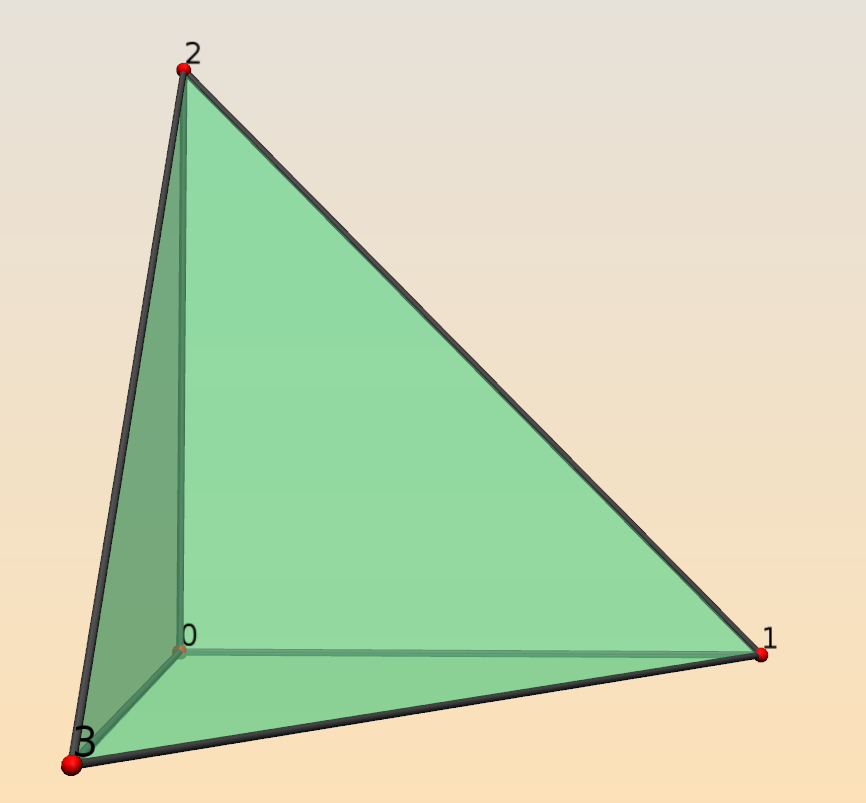
\includegraphics[width=1.0\textwidth]{fig/simplex3.png}
\end{center}
\end{column}
\end{columns}
\end{frame}
